\chapter{Analyse der Anforderungen}\label{cha:anforderungen}
In diesem Kapitel geht es um die Anwendung des Modulsystems auf die Renew Applikation. Dabei soll die Umsetzung der Theoretischen Konzepte innerhalb der Applikation, die sich Langfristig bewährt hat, unverändert bleiben und zusätzlich mit den Modulsystem Eigenschaften ausgestattet werden. \bigbreak


Die initiale Entwicklung von Renew begann mit einer monolithischen Architektur. Diese erfüllte die nötigen Anforderungen, einengte sich jedoch nicht für Entwickler mit geringem Kenntnis der Gesamtarchitektur und der darunterliegenden theoretischen Konzepten. Daher wurde eine Plugin-Architektur aufgesetzt, die es ermöglichte Studenten Renew mit Logik und Plugins zu erweitern. Diese Trägt bereits den Gedanken der \textit{Modularisierung} in sich, da die Gesamtarchitektur in Bestandsteile zerlegt und mit einander entkoppelt verknüpft wurden. Mit der Einführung des Modulsystems wird der nächste Schritt in Richtung erweiterbare und zusammen setzbare Systeme vorgenommen. \bigbreak


Dieses Kapitel diskutiert den Einfluss des Java Modulsystem auf Renew und die derzeitige Plugin-Architektur. Des weiteren werden Anforderungen erfasst, die der modularisierte Renew Prototyp erfüllen müsste um unserer Vision der Implementation zu entsprechen. 


\section{Motivation}\label{sec:motivation}

Es gibt mehrere Gründe warum Renew die Migration auf das Modulsystem durchführen sollte. Im Folgenden werden die wesentlichen Gründe, die für die Migration sprechen diskutiert.  


\subsection{Verkürzter Entwicklungszyklus}\label{sub:vez}

Die Aufteilung einer monolithischer Architektur auf eine Plugin-Architektur war ein großes Ereignis für Renew. Denn mit der Zerlegung der Gesamtarchitektur, wurde die Komplexität auf die entstandenen Komponenten aufgeteilt und erlaubte eine mühelose Weiterentwicklung der Applikation über die Plugins. \bigbreak


Obwohl die Renew Plugin-Architektur lange im betrieb blieb, hatte das Plugin-System die Codebasis umorganisiert ohne diese zu verändern. Diese führt zu alten, unverständlichen Code aus der Java 1.4 (2002) Version, mit dem viele Konzepte und Architektur Entscheidungen getroffen wurden. Nach fast 18 Jahren Betrieb altert die Codebasis sowie die Ideen und Konzepte für die Umsetzung ihrer Funktionalität. Besonders konfus und aufgebläht können Funktionsumsetzungen erscheinen, die heute von Java 12 in ein paar Zeilen gelöst werden können. Der zügiger und rapider Wandel der Software Paradigmen und deren optimaler Einsatz in der Software Architektur ist ein Teil des Fortschritts und kann nicht ignoriert werden. 


Daher ist die Modularisierung und dessen Anforderung an die Struktur und Inhalt ein wichtiges Ereignis für den Renew Lebenszyklus. Denn dieser erreicht wieder sein Ende und wird mit dem Modularisierungsschritt zurückgesetzt. \bigbreak


Renew's Entwicklungseinheit ist das Plugin. Diese repräsentiert ein bestimmtes Feature mit einen eigenen Lebenszyklus, wie zum Beispiel ein Formalismus, Simulator oder Fenster Management Plugin. Diese müssen Daten entgegennehmen, diese verarbeiten und wieder ausgeben. Demzufolge bündelt ein Plugin mehrere Fähigkeiten, die zusammen ein Feature verkörpern. Somit können Codeänderungen an mehreren Stellen im Plugin das Verhalten des Plugins beeinträchtigen und müssen auf das Gesamtverhalten getestet werden. Mit der Einführung der Module, kann das Plugin in kleinere Einheiten zerlegt werden, die anschließend eine gekapselte Teilfunktionalität des Plugins in sich tragen. Diese sind klein, leicht änderbar, ersetzbar und besitzen einen eignen Lebenszyklus. Somit verkürzt sich der Entwicklungsdauer einer Änderung und bietet eine Möglichkeit kooperativ und parallel an einem Plugin zu arbeiten. 


Demnach erweitert die Modularisierung den Renew Kontext und erlaubt das Entwickeln von Plugins in Rahmen eines Studenten Projekts, indem Teilaufgaben eines Plugins auf Module zerlegt und parallel von Studenten bearbeitet werden können. Darüber hinaus ist das Zusammenführen der Ergebnisse eine konfliktfreie Angelegenheit und bedarf keine komplette Gruppenaufmerksamkeit, um die passenden Codeblöcke für die Gesamtfunktionalität auszuwählen, da es so gut wie keine Überschneidung in der Aufgabenimplementation sich bilden kann. Somit profitiert Renew von den kurzen Entwicklungszyklen der Module und deren unproblematischen Verknüpfungseigenschaften. 


\subsection{Code-Bausteine}\label{sub:cbs}


Eine der wichtigsten Fähigkeiten eins Entwicklers, ist die Beherrschung der Komplexität. Diese führt zu sauberen, lesbaren, wartbaren Code und erweitert den Lebenszyklus einer Software um ein Vielfaches. Um dieses Kompetenz zu meistern bietet das Modulsystem von Java unterstützende Werkzeuge, die den erstellten Code organisieren und strukturieren, um ein langlebiges Ergebnis zu erzielen. 


Da Renew das Produkt vieler Abschluss-, Projekte- und Doktorarbeiten ist, durch die die Software ihre Gestalt annimmt, gibt es diverse Beschäftigte mit eigenen Zielen und Interessen. Daher ist eine allgegenwärtige, globale Strukturanforderung, die jedem Entwickler bekannt ist und an die gehalten werden muss, ein erstrebenswerte Charakteristik. 


Die im Kapitel \ref{cha:modularisierung} vorgestellten Moduleigenschaften beschreiben die von dem Java Modulsystem eingesetzten Richtlinien für die saubere Softwareentwicklung und erzwingen ein Still der fein granulierte Code-Bestandteile, die kombiniert eine Softwaresystem darstellen. An erster Stelle verhindert dieses Vorgehen den sogenannten \textit{Spaghetti Code}, der Funktionsübergreifende Anpassungen trifft und den Überblick über den Zusammenhang der Gesamtarchitektur unscharf erscheinen lässt. 


Module erschweren den \textit{Spaghetti Code}, indem Mehraufwand für die Kommunikation zwischen den Modulen erbracht werden muss und machen das unsaubere Arbeiten unattraktiv. Somit dienen Module als Grenzen für den Entwicklungsrahmen eines Features und engen den Bearbeitungs- und Betrachtungsraum für den Entwickler ein. Daraus ergibt sich ein Softwarepaket, der unabhängig von den Senior-Entwicklern verstanden, genutzt und angepasst werden kann, da der Aufbau nicht mehr in dem Wiki, Readme oder beim Entwickler selbst verankert, sondern direkt in der Codebasis integriert ist. 


Demzufolge profitiert Renew von der Modularisierung, indem sich immerfort wechselnden Akteur eine saubere Codebasis hinterlassenen, die für den nächsten Absolventen sowie den wissenschaftlichen Mitteearbeitern viel Zeit erspart. \bigbreak


Aus einer sauberen Umsetzung folgen saubere Code-Bausteine, die wiederverwendet werden können. Diese Eingenschaft der Module bringt ein wesentlich Vorteil beim Optimieren der Renew Applikation, indem kontextbezogen Module ausgetauscht werden können, um ein besseres, lokales Erlebnis zu erzielen. Zum Beispiel können zielgerichtet ausgewählte Plugins für die Erfüllung einer speziellen Aufgabe, wie das Validieren von P/T-Netzen, ein besseres Ergebnis abliefern, indem ein für diesen Anwendungsfall angepasste Verarbeitungsalgorithmus angewandt wird. Dieser ist natürlich in einem Modul gekapselt und besitzt Schnittstein identisch zu seinem Vorgänger. Auf diese Weise kann eine große Anzahl an Modulen mit gleicher Funktion und unterschiedlicher Zielsetzung erstellt werden, die in einem Modulkatalog verwaltet und bei bedarf ausgetauscht werden können. \newpage


\subsection{Bereit für Innovation} \label{sub:moderner_zustand}
% Ziel
Der zeitgemäße Zustand einer Applikation ist eine Zeichen hoher Qualität und reflektiert enorme Ansprüche an den Betrieb der Applikation. Diese kann geschäftskritische Qualitäten tragen, die den marktführenden Vorteile bringen und sich gegen die Konkurrenz durchsetzen. Um den Vorsprung zu sichern, ist eine \textit{vorausschauende} Flexibilität gefragt. Mithilfe dessen die Applikation in der Lage ist, mit minimalen Aufwand, an die führenden Technologien anzuknüpfen. 

% Trends 
Die Aktuell führenden Trends beschäftigen sich mit der verteilten und wiederverwendbaren Softwareumsetzungen, die ständig an Komplexität gewinnen und trotzdem leicht Beherrschbar bleiben muss. Diese beschreiben Ansätze wie gewisse Ziele erreicht werden können und setzen Grundvoraussetzungen zum erreiche dieser Ziele. Dementsprechend muss Renew bestimmte Grundvoraussetzungen erfüllen um die Vorteile der Trends zu Nutzen und den Schritt mit dem Fortschritt zu halten.  \bigbreak


% Docker  
Zum Beispiel wäre die Docker Umgebung für Renew eine willkommene Erweiterung, mit der interne Bestandsteile distributiv betrieben werden können. Somit wäre die Ausführung von Renew nicht mehr an eine Maschine gebunden und kann bei Bedarf horizontal skaliert werden. Im Folgenden stellt sich die Frage: welche interne Strukturen von Renew müssen individuell behandelt und anschließend kooperativ zusammengeführt werden. Auf diese Frage gibt es keine pauschale Antwort, jedoch ist es klar, dass die Plugins von Renew Feingranular betrachtet werden müssen, um sich ein Bild der Verarbeitungskette zu erstellen und diese unseren Bedürfnissen anzupassen. \bigbreak

% Microservice  
Renew auf verschieden Hardwareknoten zu verteilen ist nur der erste Schritt der distributiven Ausführung. Es fehlt die Koordination zwischen den Knoten, die die Verarbeitung koordinieren und die Ergebnisse zusammenfassen. Somit gibt es eine weitere Technologie, die sich dieser Aufgabenstellung widmet: Der Mikroservice Architekturansatz, der sich um die Koordination und den Zusammenspiele von \textit{Applikationsschwärme} kümmert. \bigbreak

% Fazit 	
Mit Hilfe der Mikroservicearchitektur und der Docker-Umgebung wäre die distributive Ausführung von Renew erreichbar, doch zuerst muss Renew den aktuellen Stand der Technologie entsprechen und demzufolge das Modulsystem von Java integriert wird.  


\section{Ausgangssituation} \label{sec:ausgangssituation} 

Renew ist in mehr als 60 Plugins aufgeteilt, die für sich allein stehende Projekte repräsentieren. Jedes Projekt besitzt eine \textit{buidl.xml} und wird mit dem übergeordneten Stamm \textit{build.xml} Script zusammengeführt. Die XML-Scripte werden von dem \textit{Apach Ant} Werkzeug evaluiert, kompiliert und zusammengeführt. In folge dessen entsteht ein \textit{jar} Archiv für jedes Plugin-Projekt. Diese werden in eine bestimmte Orderstruktur für die Ausführung aufbereitet, die sich aus dem \textit{config, plugins} und \textit{libs} Verzeichnis zusammensetzt. 
\bigbreak

Der innere Aufbau jedes Plugins benötigt eine besondere Konfigurationsdatei, nämlich die \textit{plugin.cfg}. Diese beschreibt für die Ausführung nötige Plugin-Abhängigkeiten und wird von den internen Plugin-Manager verwaltet, der für die richtige Ordnung beim Laden jedes einzelnen Plugins aus dem \textit{plugins} Verzeichnis sorgt. Somit sind die \textit{plugin.cfg} Dateien ein guter Startpunkt für die Evaluation einer minimalen und lauffähigen Renew Konfiguration. 
\bigbreak

Für die Evaluation der minimale Konfiguration starten wir aus dem \textit{Gui}-Plugin und arbeiten uns die Plugin-Hierarchie der \textit{plugin.cnf} herunter bis der komplette Graph aufgebaut ist.

\begin{figure}[h!]
  \centering
  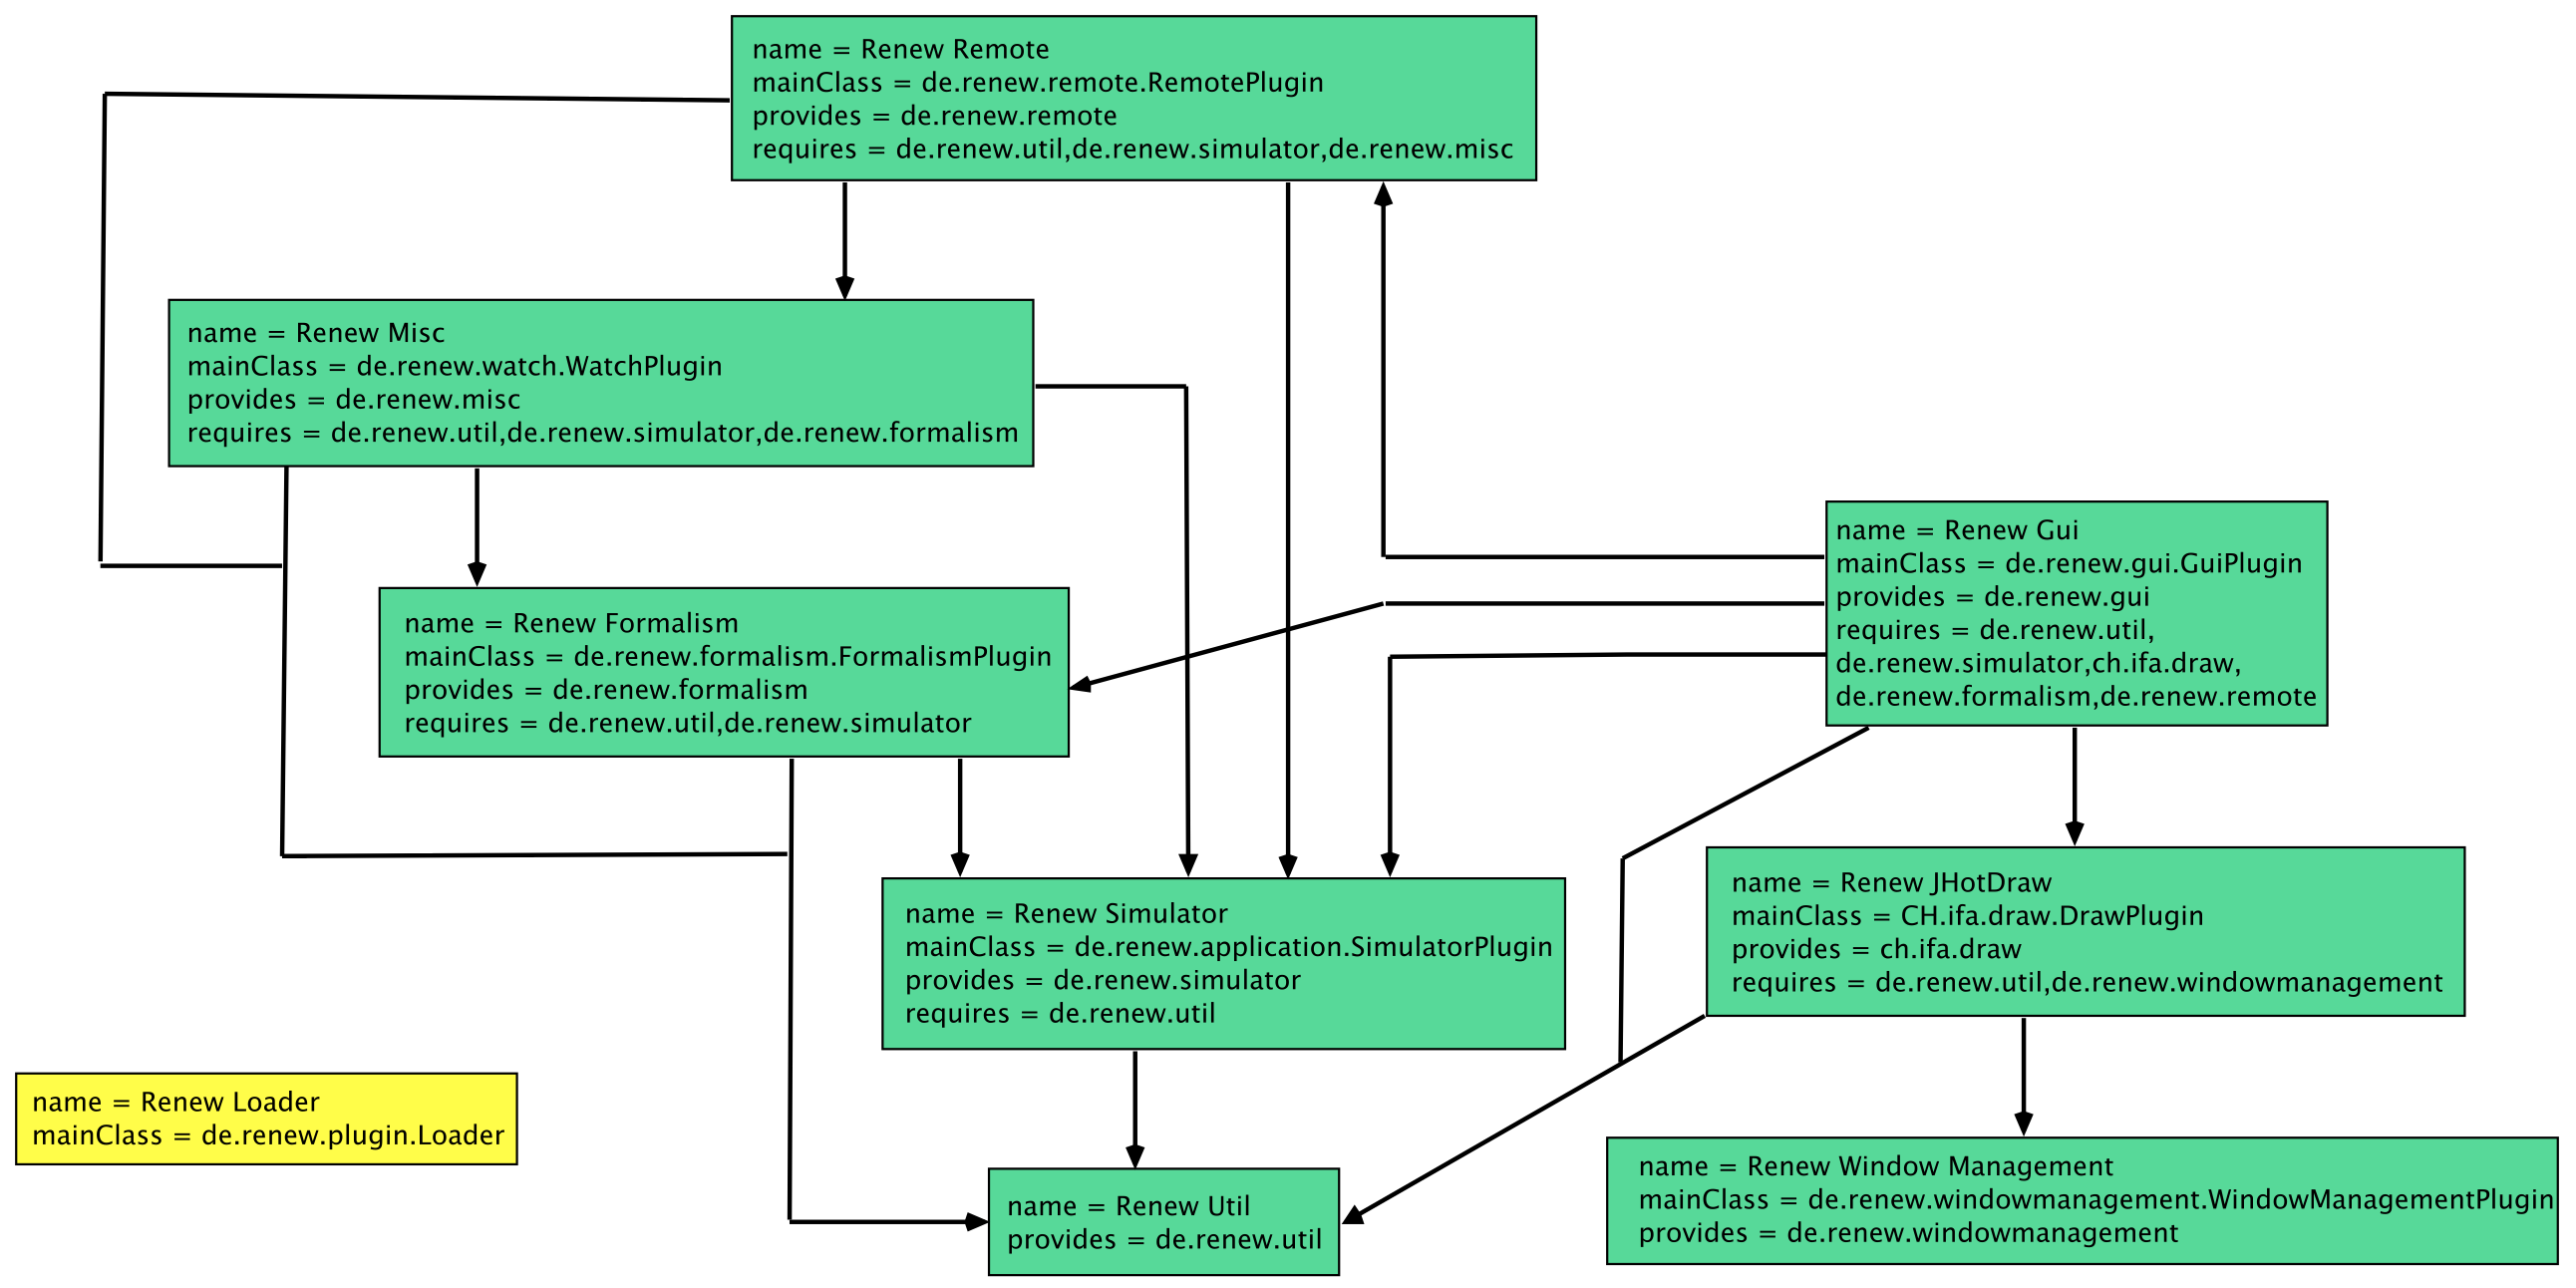
\includegraphics[width=\textwidth]{material/images/plugin_deps.png}
  \caption{Gui Plugin-Abhängigkeiten}
  \label{fig:plugin_deps}
\end{figure}

Die in der Abbilde \ref{fig:plugin_deps} repräsentierten Zusammenhängen reflektieren die von den Entwickler abgestimmten Laufzeitabhängigkeiten, die einen groben Überblick über die nötigen Plugins verschaffen. Diese können zur Laufzeit alle benötigen Daten und Klassen enthalten, jedoch tragen sie keine Aussage über Abhängigkeiten während der Kompilation. Demgemäß kann zusätzlicher Code sowie Plugins benötigt werden. 


\section{Auswirkung} \label{auswirkung}

Die Folgeerscheinung der Modularisierung unterbindet zahlreiche Entwicklungsschwächen, wie \textit{Zyklen}, \textit{Split Packages} und antiquierte API's. Diese sollen mit der Migration aufgelöst,reorganisiert und nachgerüstet werden, um einen kompelierfähigen Zustand erreichen zu können.

\subsubsection{Zyklenfrei} 
Mit den Zyklen-freien Plugins werden Abhängigkeiten aufgelöst, die sich an falschen stellen befinden und mehr als eine Aufgabe Plugin übergreifend lösen möchten. Diese haken sich in den Betrieb der unmittelbar angrenzenden Komponenten ein und machen sich unverzichtbar für die Ausführung der Software. Die minimale Renew Version hat keine Laufzeitzyklen und erfüllt somit das Kriterium der Zyklenfreiheit, nichtsdestotrotz sind diese in der erweiterten Version nicht ausgeschlossen.

\subsubsection{Split Packages}
Der Mangel der \textit{Split Packages} wird in einer Plugin-Architektur mit großer Wahrscheinlichkeit einträten, da Plugins aus dem gleichem Kontext, wie \textit{Navigator} oder \textit{NavigatorGit}, den selben \textit{de.renew.navigator.*} Namensraum beanspruchen. Dieses führt zum Fehler beim auflösen der benötigten Klasse und verhindert das Hochfahren der Applikation. 

\subsubsection{Schnittstellen}
Die Plugin.cfg beschreibt die Abhängigkeit der Module unter einander, jedoch ist diese Informantin unvollständig, denn es fehlt dieser die Information über Schnittstellen des Plugins und dafür ausgelegten Pakete. Infolgedessen hat der Entwickler keine andere Möglichkeit als auf gewünschte Plugin-Funktionen direkt zu zugreifen ohne einen festen Vertrag über die Kommunikation einzugehen. Somit kann jede Änderung und Aktualisierung innerhalb eines Plugins zum unerwarteten Verhalten seiner Nutzer führen. Im Gegensatz zu den \textit{Plugin.cfg} führt die \textit{module-info.java} eine Liste an exportierten Paketen sowie importierten Modulen. Dies erlaubt nicht nur das Verständnis der benötigten Module, sondern unterstützt den Entwickler durch klar definierte Schnittellen, die mit dem Schlüssel \textit{exports} deklariert sind.

\subsubsection{Homogene Umgebung}
% laufzeitumgebung = kompelierumgebung 
\subsubsection{Service Loader} 


\newpage

+ Keine Zyklen 
+ keine split packages

+ sofort erkennbanre abhängigkeiten
+ sofort erkennbare einsatzorte 
+ laufzeitumgebung = kompelierumgebung 

+ düne laufzeitanforderungen (braucht nicht alle libs)
+ jmod und kein Verzeichniss 

	- was sind willkommene Eingenschaften 
	- was wird besser gemacht 
	- welche Mängel werden behoben 
	- welche Nebenwirkungen hat das Modulsystem: Positiv oder Negativ. 

\section{Anforderungen} \label{sec:anforderungen}
- Anforderungen an System 
	- was soll der Prototyp leisten 
	- welche spezifische Dinge möchte ich behandeln 
	- in welche Richtung und aus welcher Perspektive möchte ich migrieren 
	- begründe den Migrationsansatz 
	- eine Anforderungsmenge die von mehreren Prototypen umgesetzt wird 



